\section{Reference Time Cuts} \label{sec:reftime}

Figure~\ref{fig:reference_time_cartoon} illustrates the relationship
between a detector signal and the internal clocks of the CAEN 1190 TDCs that
determine the timing resolution of measurements in Hall C.
An L1 pretrigger (see Section~\ref{sec:daq}) that initiates read-out
in a ROC latches onto the leading edge of the next cycle of an 1190's
\SI{40}{\mega\hertz} clock.
As a result, this digitized pretrigger time can only be known to have been
received within the \SI{25}{\nano\second} window between that
\SI{40}{\mega\hertz} cycle and the previous cycle.
Pretriggers also have an intrinsic \SI{4}{\nano\second}
jitter\footnote{A small, irregular variation in an otherwise periodic signal.},
meaning that raw TDC signals can only be known to within
\SI{\sim29}{\nano\second}.
To improve the timing resolution, the DAQ sends a delayed copy of the
pretrigger, called a \textit{reference time}, to the TDC.
The reference time latches onto the leading edge of the 1190's
\SI{10}{\giga\hertz} clock (accurate to \SI{0.1}{\nano\second}), and initiates
read-out of the full TDC spectrum (a lookback window of a few
\si{\micro\second}).
All modules in a given ROC share the same reference time.
Therefore, subtracting the raw TDC time (synced to the \SI{40}{\mega\hertz}
clock) from the reference time (synced to the \SI{10}{\giga\hertz} clock),
the timing resolution can be improved to approximately \SI{0.1}{\nano\second}.
This reference time subtraction is performed offline during \textit{hcana}
replay.


\begin{figure}[!h]
    \centering
    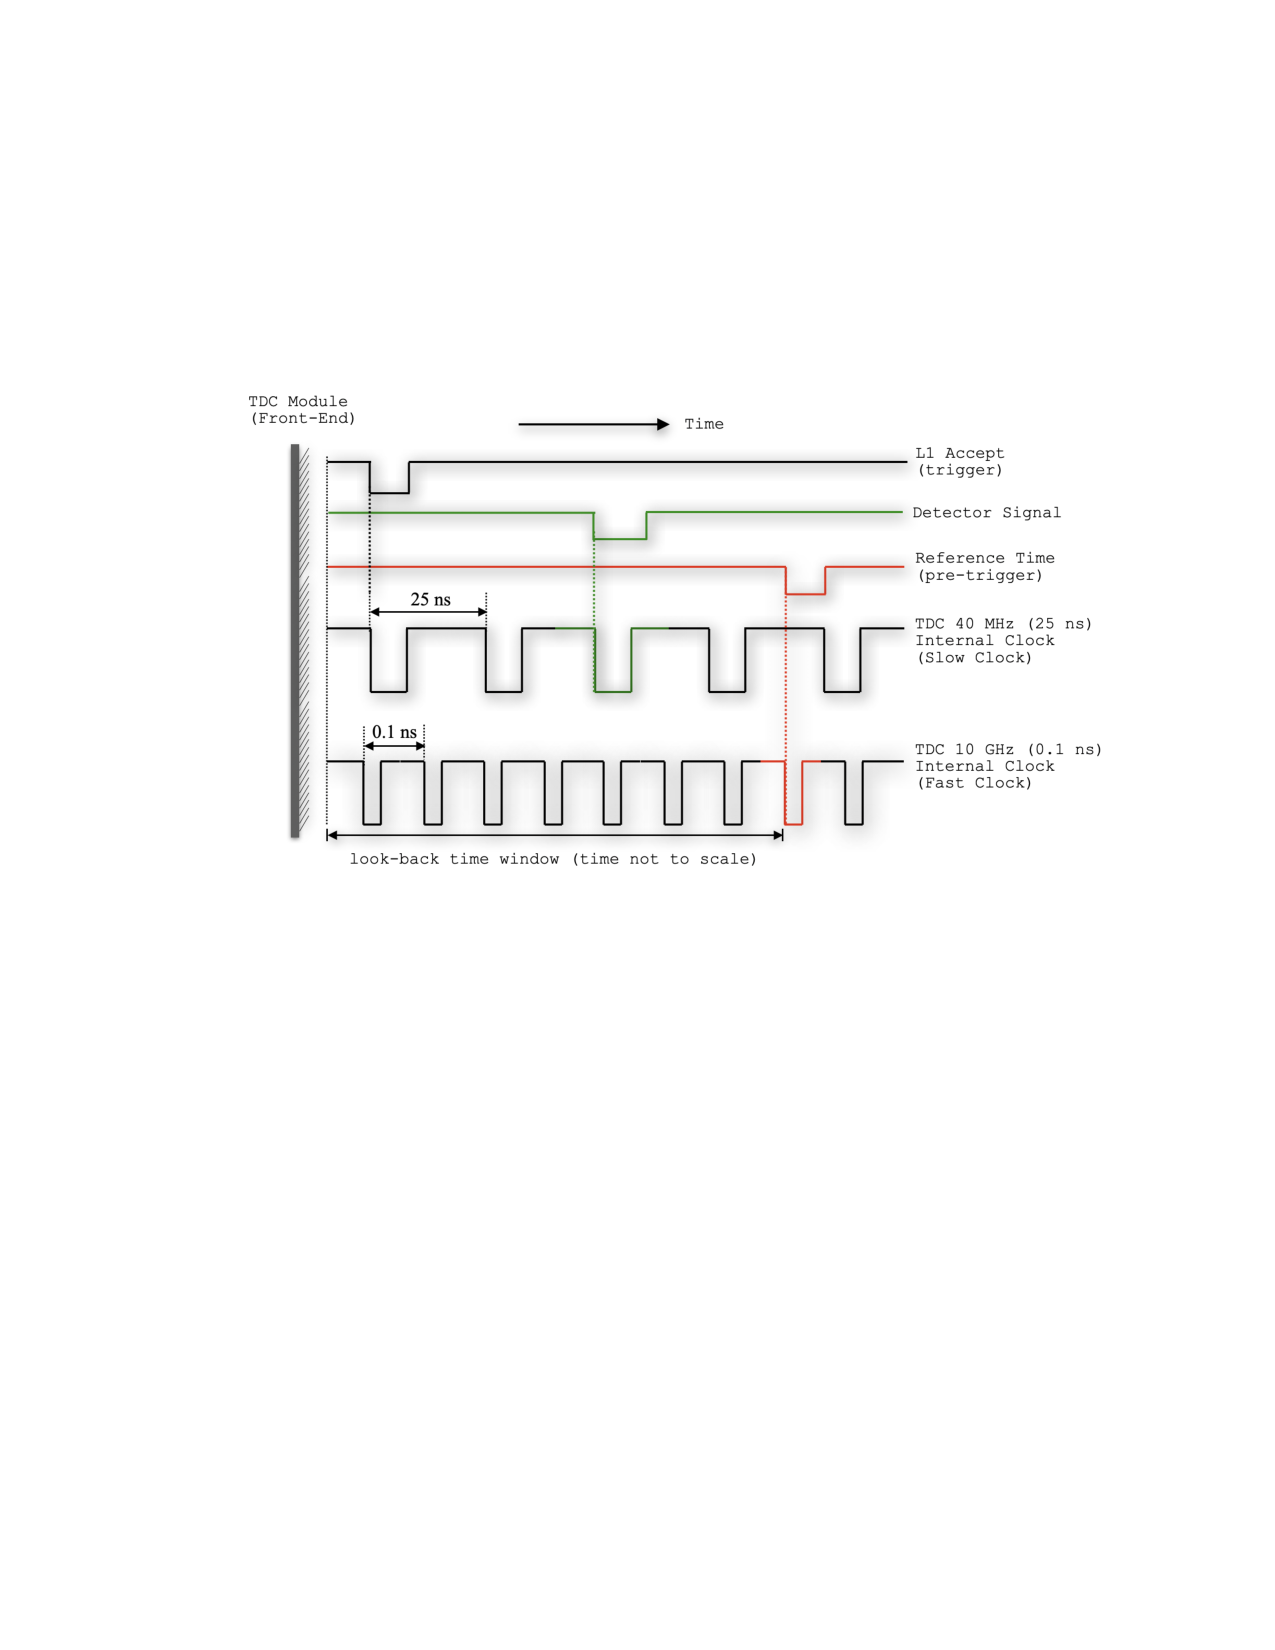
\includegraphics[width=1.0\textwidth]{chap4/yero_reftime.pdf}
    \caption{
            A cartoon illustrating the synchronization of a detector signal
            with a CAEN 1190 TDC's internal \SI{4}{\mega\hertz} and
            \SI{10}{\giga\hertz} clocks. Figure reproduced from Carlos Yero's
            PhD thesis~\cite{Yero_2020}.
            }
    \label{fig:reference_time_cartoon}
\end{figure}


% TODO: ref time cut example figure
As shown in Figure,
true physics events will lie within a range of X raw TDC channels.
Background events will have occurred earlier in the lookback window, and must
be prevented from being chosen as the reference time.
To accomplish this, \textit{hcana} uses reference time cuts defined in
the parameter files.


\section{Detector Time Window Cuts}
As with reference time selection, care must be taken to avoid background hits
in the fADC spectra.
The distribution of the differences between the fADC pulse times and
reference-time-subtracted TDC times for a given PMT in a detector should
be a narrow peak with a width determined by the resolutions of the TDCs
and fADCs.

\section{Dead Time} \label{sec:deadtime}

\section{Coincidence Time}
